%%%%%%%%%%%%%%%%%%%%%%%%%%%%%%%%%%%%%%%%%
% Journal Article
% LaTeX Template
% Version 1.3 (9/9/13)
%
% This template has been downloaded from:
% http://www.LaTeXTemplates.com
%
% Original author:
% Frits Wenneker (http://www.howtotex.com)
%
% License:
% CC BY-NC-SA 3.0 (http://creativecommons.org/licenses/by-nc-sa/3.0/)
%
%%%%%%%%%%%%%%%%%%%%%%%%%%%%%%%%%%%%%%%%%

%----------------------------------------------------------------------------------------
%	PACKAGES AND OTHER DOCUMENT CONFIGURATIONS
%----------------------------------------------------------------------------------------

\documentclass[twoside]{article}
\usepackage{graphicx}

\usepackage[sc]{mathpazo} % Use the Palatino font
\usepackage[T1]{fontenc} % Use 8-bit encoding that has 256 glyphs
\linespread{1.05} % Line spacing - Palatino needs more space between lines
\usepackage{microtype} % Slightly tweak font spacing for aesthetics

\usepackage[hmarginratio=1:1,top=32mm,columnsep=20pt]{geometry} % Document margins
\usepackage{multicol} % Used for the two-column layout of the document
\usepackage[hang, small,labelfont=bf,up,textfont=it,up]{caption} % Custom captions under/above floats in tables or figures
\usepackage{booktabs} % Horizontal rules in tables
\usepackage{float} % Required for tables and figures in the multi-column environment - they need to be placed in specific locations with the [H] (e.g. \begin{table}[H])
\usepackage{hyperref} % For hyperlinks in the PDF

\usepackage{lettrine} % The lettrine is the first enlarged letter at the beginning of the text
\usepackage{paralist} % Used for the compactitem environment which makes bullet points with less space between them

\usepackage{abstract} % Allows abstract customization
\renewcommand{\abstractnamefont}{\normalfont\bfseries} % Set the "Abstract" text to bold
\renewcommand{\abstracttextfont}{\normalfont\small\itshape} % Set the abstract itself to small italic text

\usepackage{titlesec} % Allows customization of titles
\renewcommand\thesection{\Roman{section}} % Roman numerals for the sections
\renewcommand\thesubsection{\arabic{subsection}} % Roman numerals for subsections
\titleformat{\section}[block]{\large\scshape\centering}{\thesection.}{1em}{} % Change the look of the section titles
\titleformat{\subsection}[block]{\large}{\thesubsection.}{1em}{} % Change the look of the section titles

\usepackage{fancyhdr} % Headers and footers
\pagestyle{fancy} % All pages have headers and footers
\fancyhead{} % Blank out the default header
\fancyfoot{} % Blank out the default footer
\fancyhead[C]{PPGEB - FEELT - UFU $\bullet$ 2013/2} % Custom header text
\fancyfoot[RO,LE]{\thepage} % Custom footer text

\usepackage[utf8]{inputenc}
\usepackage{graphicx}
\graphicspath{{imgs/}}

\usepackage{listings}
\usepackage{xcolor}

\lstdefinestyle{sharpc}{language=[Sharp]C, frame=lr, rulecolor=\color{blue!80!black}, breaklines=true}

%----------------------------------------------------------------------------------------
%	TITLE SECTION
%----------------------------------------------------------------------------------------

\title{\vspace{-15mm}\fontsize{24pt}{10pt}\selectfont\textbf{Implementação de um sistema de auto completar em um software de CAA para pacientes com limitação motora severa}} % Article title

\author{
\large
\textsc{CURTT JR., FERREIRA L.C.V., LIMA M.A.B., MARIANO D.T.G., NAVES E.L.M.}\\[2mm] % Your name
\normalsize Laboratório de Engenharia Biomédica\\\normalsize Núcleo de Tecnologias Assistivas\\\normalsize Universidade Federal de Uberlândia\\ \normalsize Uberlândia-MG, Brasil \\ % Your institution
\normalsize {jrcurttjr@msn.com, lcv.ferreira@yahoo.com.br, borba.lima@hotmail.com, dtgmariano@gmail.com} % Your email address
\vspace{-5mm}
}
\date{}

%----------------------------------------------------------------------------------------

\begin{document}

\maketitle % Insert title

\thispagestyle{fancy} % All pages have headers and footers

%----------------------------------------------------------------------------------------
%	ABSTRACT
%----------------------------------------------------------------------------------------


\begin{abstract}
\noindent
Uma das principais formas de socialização que o ser humano possui é a fala, que lhe garante o entendimento por outros, de seus anseios e desejos. Desta forma distúrbios neurológicos como a esclerose lateral amiotrófica (ELA) ou outras doenças musculares progressivas, conduzem frequentemente esses indivíduos à paralisia motora, inclusive com prejuízo a fala. Sendo assim este trabalho busca analisar a ferramenta EDITH, software utilizado para a comunicação de pacientes em estágio avançado de ELA, e propor a introdução de um sistema de auto completar junto a esta ferramenta. Para isto foi utilizado, .......... 
\end{abstract}

%----------------------------------------------------------------------------------------
%	ARTICLE CONTENTS
%----------------------------------------------------------------------------------------

\begin{multicols}{2} % Two-column layout throughout the main article text

\section{Introdução}
\subsection{Panorama das tecnologias assistivas}
Uma das principais formas de socialização que o ser humano possui é a fala, que lhe garante o entendimento por outros, de seus anseios e desejos. No Brasil, conforme o censo realizado em 2010 pelo IBGE existe cerca de 45,6 milhões de pessoas com deficiência, o que representa 23,9% da população brasileira, sendo que grande parte destas pessoas possui um ou mais tipos de deficiência, podendo ser física, visual, auditiva, intelectual ou de comunicação1.
Ao analisar a vida cotidiana do ser humano, é possível dizer que uma gama de fatores podem influenciar suas atitudes e atividades diárias, seja no trabalho ou na vida social, para isto se faz necessário englobar uma análise ergonômica de suas atividades, para saber como estas situações, seja de forma positiva ou negativa, afetam o indivíduo nas questões físicas, sociais ou psicológicas.  A palavra Ergonomia é de origem grega sendo, ergo significando tarefa, por extensão trabalho, e nomos normas, regras2.
Assim sendo ergonomia pode ser definida como uma abordagem científica que se fundamenta em conhecimentos interdisciplinares das ciências humanas para, de um lado, compatibilizar os produtos e as tecnologias com as características dos usuários e, de outro, humanizar o contexto sociotécnico de trabalho, adaptando-o tanto aos objetivos do sujeito e/ou grupo, quanto às exigências das tarefas3; 4. Com o estudo da ergonomia surge uma área de grande importância para a adaptação do deficiente à vida em sociedade, que é a tecnologia assistiva (TA), que é utilizado para identificar todo o arsenal de recursos e serviços que contribuem para proporcionar ou ampliar habilidades funcionais de pessoas com deficiência e consequentemente promover vida independente e inclusão. Podendo ser definido ainda como, uma ampla gama de equipamentos, serviços, estratégias e práticas concebidas e aplicadas para minorar os problemas funcionais encontrados pelos indivíduos com deficiências5.
Faz-se necessário realizar ou promover a pesquisa e o desenvolvimento, bem como a disponibilidade e o emprego de novas tecnologias, inclusive as tecnologias da informação e comunicação, ajudas técnicas para locomoção, dispositivos e tecnologias assistivas, adequados a pessoas com deficiência, dando prioridade a tecnologias de custo acessível6.
Por assim ser, há a necessidade de se desenvolver instrumentos que facilitem à socialização destas pessoas com deficiência, seja através da forma mais simples ou da forma mais complexa (cartilhas de comunicação, ambientes adaptados, softwares, hardwares, etc.) estes instrumentos são conhecidos como tecnologia assistiva7.
Desta forma, tecnologia assistiva é qualquer produto, instrumento, equipamento ou sistema técnico utilizado por uma pessoa incapacitada, que se destina a prevenir, compensar, monitorizar, aliviar ou neutralizar a incapacidade8.
Os recursos e serviços de tecnologia assistiva são organizados ou classificados de acordo com objetivos funcionais a que se destinam, tais como mobilidade, adequação postural, comunicação, recursos para cegos ou pessoas de baixa visão, para surdos ou pessoas com perdas auditivas, instrumentos que promovam independência em atividades da vida diária, recursos para educação, recreação, acessibilidade arquitetônica, adaptações de veículos, recursos para acesso ao computador, órteses, próteses e outros9.
Recursos de comunicação podem ser dos mais variados tipos. Projeta-se e constrói-se um recurso considerando as habilidades do usuário com o objetivo de ajudá-lo a superar sua deficiência. Um recurso após ser desenvolvido e aplicado poderá ser então aperfeiçoado, considerando as dificuldades de adaptação do indivíduo9. 
Para atender pessoas sem fala, sem escrita funcional ou em defasagem entre sua necessidade comunicativa e sua habilidade em falar e/ou escrever, são utilizados recursos conhecidos como comunicação aumentativa e alternativa (CAA). A CAA serve para expressar suas questões, desejos, sentimentos, entendimentos. A alta tecnologia dos vocalizadores (pranchas com produção de voz) ou o computador com softwares específicos garantem grande eficiência à função comunicativa5.
Distúrbios neurológicos como a esclerose lateral amiotrófica (ELA) ou outras doenças musculares progressivas, conduzem frequentemente esses indivíduos à paralisia motora, inclusive com prejuízo a fala. Tornam-se, portanto, altamente limitados para suas atividades, inclusive com privação de suas vontades, devido à perda de comunicação.
Esta patologia atinge cerca de 1 a 3 novos casos por cada 100,000 habitantes anualmente, tendo uma prevalência detida entre os 3 e os 7 por 100,000 habitantes/ano. Ainda por razões desconhecidas, o sexo masculino tem um predominância ligeiramente superior quando comparado com o feminino, com uma proporção M:F de 1,5:1 10. Habitualmente a idade média de aparecimento da doença ocorre entre os 55-65 anos de idade, embora em  alguns casos, cerca de 5% possa manifestar-se a partir da segunda década de vida11.
Para alguns desses indivíduos o sistema de escaneamento é o único modo de acesso à comunicação verbal ou escrita. Esses fundamentos têm sido utilizados desde o início da década de 80: através de um sistema de varredura luminosa, um item é marcado na tela e então selecionado por um clique. A principal desvantagem desse método é a lentidão na comunicação com uma velocidade média de escaneamento entre 0,2 a 6 segundos7.

\subsection{Edith}
Uma ferramenta com esse objetivo é o EDITH (acronismo francês para Ambiente de Teleação Digital para Pessoas com Disfunções), desenvolvido na Universidade Metz, França; esse software foi originalmente desenvolvido para uma pessoa com ELA e instalado em um laptop.

\begin{figure}[H]
\label{fig:edith_menu}
  \caption{Menu do EDITH.}
  \centering
    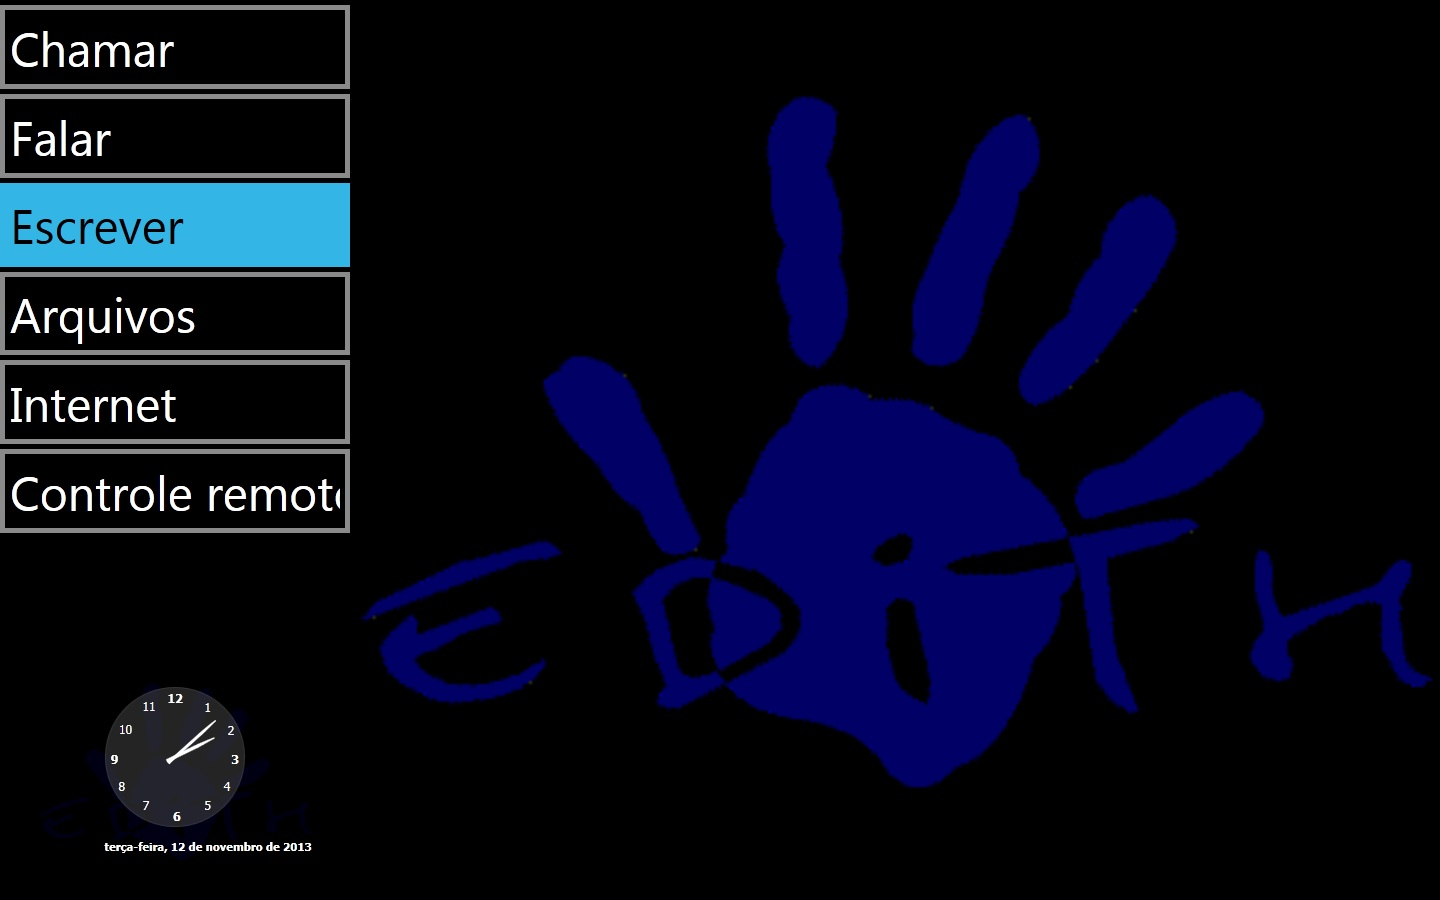
\includegraphics[scale = 0.18]{edith_menu.png}
\end{figure}

Trata-se de um sistema de auxílio à comunicação destinada a pessoas com deficiências motoras severas e que não estão aptas a se comunicarem. Ele é composto por um software que integra diversos recursos para controle de um ambiente multimídia de comunicação. Para o sistema de seleção costuma-se aplicar o modo linha-coluna (ou coluna-linha), por proporcionar um menor dispêndio de esforço físico e mental nessas ações. O sistema de seleção pode também ser sequencial, se a disponibilidade de opções não for muito ampla. 

\begin{figure}[H]
\label{fig:edith_tecladovirtual}
  \caption{Teclado virtual.}
  \centering
    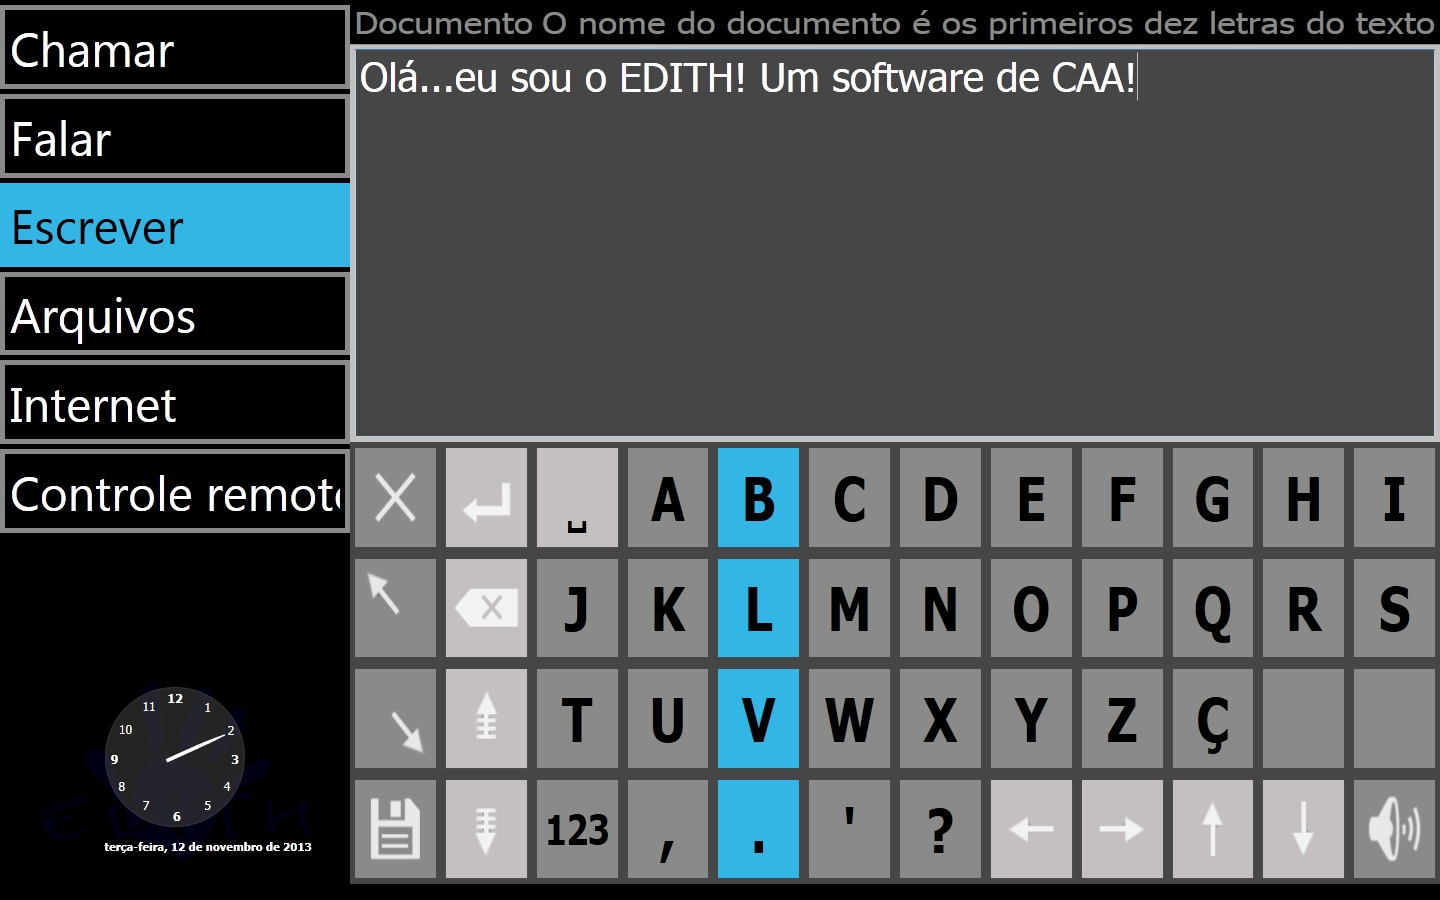
\includegraphics[scale = 0.18]{edith_tecladovirtual.png}
\end{figure}

É possível ajustar o parâmetro temporal de acordo com a personalidade e as habilidades físicas e cognitivas do usuário; pode ser diminuído quando o usuário adquirir experiência com a interface, ou aumentado, se houver deterioração da função por agravo da enfermidade. O sistema EDiTH foi projetado para computadores padrão IBM-PC e possui duas componentes principais: uma interface funcional e uma interface de configuração. A interface funcional oferece várias facilidades como avisos e chamadas sonoras do pessoal de enfermagem, leitura de textos e escrita de texto. A interface de configuração permite ao usuário ajustar a operação de diversas funcionalidades como tempo de varredura do teclado virtual, adicionar livros, filmes, músicas no banco de dados e cadastrar e-mails.

\begin{figure}[H]
\label{fig:edith_chamar}
  \caption{Módulo para chamada urgente.}
  \centering
    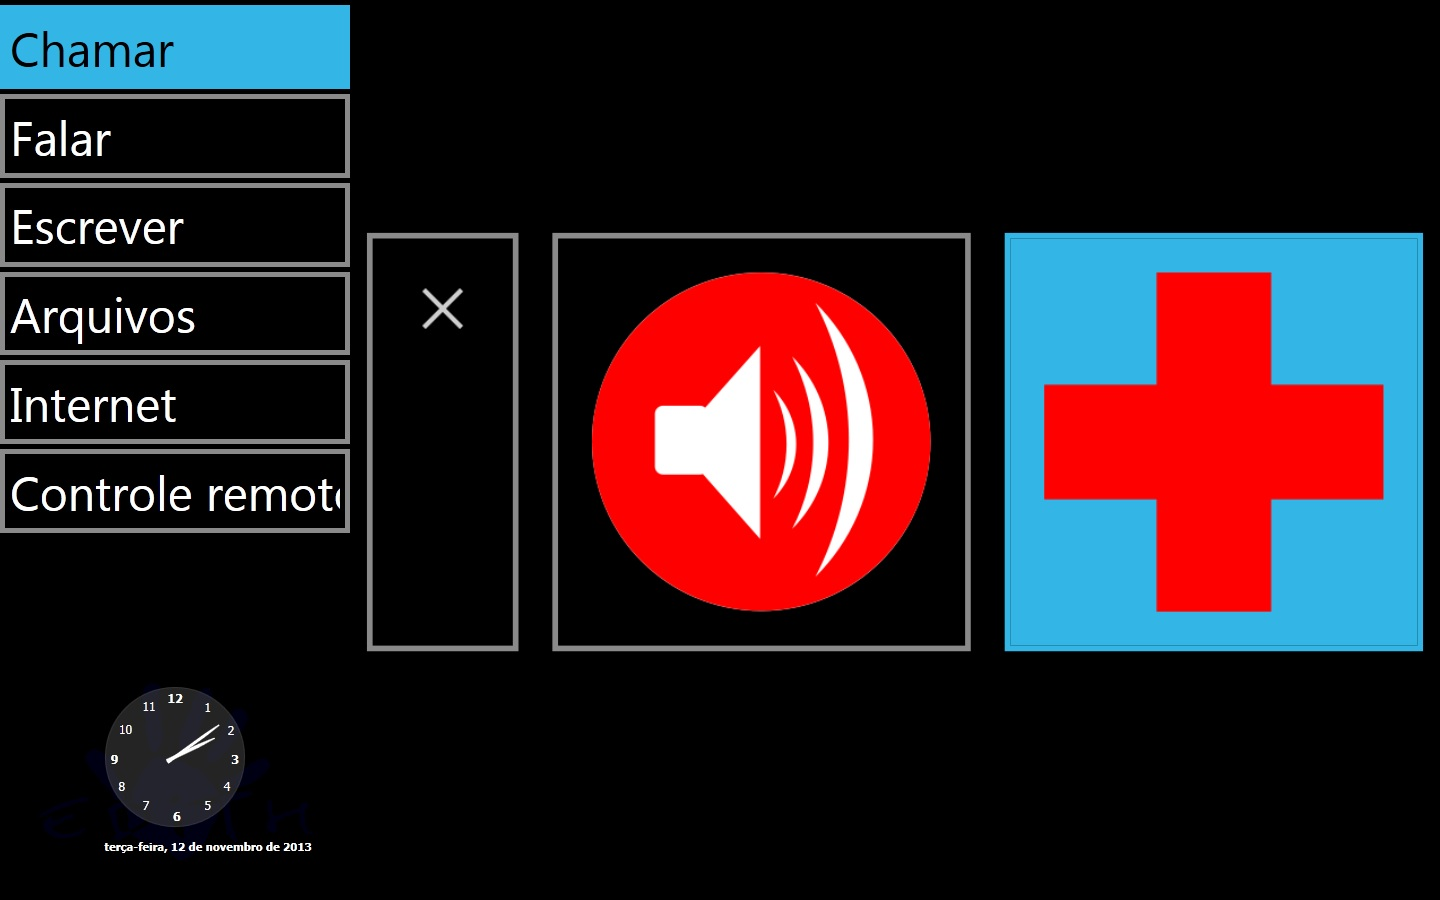
\includegraphics[scale = 0.18]{edith_chamar.png}
\end{figure}

O software foi desenvolvido na plataforma de desenvolvimento .NET da Microsoft, utilizando linguagem computacional C\# (CSharp). O aplicativo possui um gerador de registros (log) que grava as ações desempenhadas pelo usuário durante a execução do programa. O objetivo de vários pesquisadores que atuam na área de tecnologia assistiva tem sido a de aperfeiçoar esses softwares para uma melhor adaptação do usuário com a interface, permitindo menor esforço físico e melhor aproveitamento desses recursos. Indivíduos com disfunções motoras associados a distúrbios da fala frequentemente utilizam-se de recursos de comunicação como o EDITH, contudo, devido a velocidade que a escrita é executada, às vezes por limitações físicas desses pacientes, esses dispositivos tornam essa capacidade de comunicação uma tarefa de difícil execução. 


%------------------------------------------------

\section{Métodos}

Esta é uma pesquisa do tipo experimental quantitativa, Com o objetivo de melhorar a velocidade de comunicação e diminuir esforços aos usuários do software EDITH, foi introduzida ao software a ferramenta “autocompletar” a caixa de texto, de modo a diminuir a frequência de seleção dos itens do painel. Para isso serão realizados alguns testes comparando a performance do usuário utilizando o recurso auto-completar e sem o mesmo. Com base nos registros de (log) do software, serão analisados alguns dados por meio de ferramentas estatísticas.

\subsection{Desenvolvimento da ferramenta autocompletar}

\subsection{Ensaios}
Como ensaio foi proposto ao voluntário a escrita de uma frase no 


%------------------------------------------------

\section{Resultados}

%------------------------------------------------

\section{Discussão}


%----------------------------------------------------------------------------------------
%	REFERENCE LIST
%----------------------------------------------------------------------------------------

\begin{thebibliography}{99} % Bibliography - this is intentionally simple in this template

\bibitem _CEPES/IEUFU. Levantamento de Informações econômico-sociais da População Portadora de Deficiência no Município de Uberlândia-MG. UFU 2005.

\bibitem _CUNHA, A. G. Dicionário etimológico Nova Fronteira da língua portuguesa. FRONTEIRA, N. Rio de Janeiro 1982.

\bibitem _DANIELLOU, F., Ed. L’ergonomie en quête de ses principes. Débats épistémologiques. Toulouse, França: Octares Editionsed. 1996.

\bibitem _MONTMOLLIN, M., Ed. L'ergonomie. Paris, Editions La Découverte ed. 1990.

\bibitem _COOK, A. M. H., S. M. Assistive Technologies: Principles and Practices. Mosby. YEAR BOOK, I. St. Louis, Missouri 1995.

\bibitem _BRASIL. Experiências Educacionais Inclusivas. Programa Educação Inclusiva Direito à Diversidade. ESPECIAL., M. D. E. S. D. E. Brasília 2007.

\bibitem _ROCHA, L. A. D. A. D. INTERFACE MULTIMODAL APLICADA À COMUNICAÇÃO ALTERNATIVA PARA PESSOAS COM DEFICIÊNCIAS MOTORAS GRAVES. 2013.   Departamento de Engenharia Elétrica, Universidade Federal de Uberlândia, Uberlândia.

\bibitem _BRASIL. Decreto 5.296 de 02 de dezembro de 2004. FEDERAL, G. Brasília. Decreto 5.296 2004.

\bibitem _BERSCH, R. M. H., PASSERINO, L. M., BATISTA, V. J. Tecnologia Assistiva e Design na Realidade Brasileira. Anais do Terceiro Workshop Design e Materiais da UFRGS. Porto Alegre, RS 2007.

\bibitem _TURNER MR, H. O., BENATAR M, BROOKS BR, CHIO A, DE CARVALHO M, ET AL. Controversies and priorities in amyotrophic lateral sclerosis. Lancet Neurologyogy, v. 12, p. 310-322,  2013.   

\bibitem _HAUSER SL, F., AS, EUGENE B, KASPER DL, LONGO DL, JAMESON JL, LOSCALZO J. Amyotrophic Lateral Sclerosis and Other Motor Neuron Diseases. Estados Unidos da América: McGraw-Hill Companies: 358-363 p. 2010.




\end{thebibliography}

%----------------------------------------------------------------------------------------

\end{multicols}

\end{document}